%!TEX encoding = UTF-8 Unicode
% ===============================================================================
% = LaTeX Beamer Template des Arbeitsbereichs Sicherheit in verteilten Systemen
% = (c) 2016 Prof. Dr. Hannes Federrath, Uni Hamburg, Fachbereich Informatik
% = https://svs.informatik.uni-hamburg.de
% =
% = Weitgehend in Übereinstimmung mit dem Corporate Design 2016 der UHH:
% = https://www.uni-hamburg.de/beschaeftigtenportal/services/oeffentlichkeitsarbeit/corporate-design.html
% ===============================================================================
%
\documentclass[t,aspectratio=169]{beamer}
% Option t              Place text of slides at the (vertical) top of the slides.
% Option handout        Create PDF without pauses and overlay-effects.
% Option aspectratio=43 169 => 16:9, 1610 => 16:10, 43 => 4:3
\usepackage[utf8]{inputenc}
\usepackage[ngerman]{babel}
\usepackage{graphicx,xcolor}
\usepackage[T1]{fontenc} % 8-bit-characters; allows copying UTF-8 characters
\usepackage{courier}     % modifies the monospace font

% Apply theme
\usetheme{svs2021}

\title{Dangers and Prevalence of\\ Client-Side Web API Manipulations}
% \subtitle{Subtitle}
\author{Jonas Bögle de Araújo\\ \footnotesize Student ID No. 7200785}
% \institute[Uni Hamburg]{Universität Hamburg · Fachbereich Informatik}
\date{14.06.2022}

% Note: \maketitle and \tableofcontents require recompiling the document
% TODO: \pause{}
% TODO:
% motivation, what is WAM. ? ...

\begin{document}

\begin{frame}
	\maketitle
\end{frame}

\begin{frame}
	\frametitle{Agenda}
	\tableofcontents
	% Create entries with \section{} and \subsection{}
\end{frame}

\section{Introduction}
%\subsection{Goals}
%\subsection{Motivation}

\begin{frame}
	\frametitle{Introduction}
	% \framesubtitle{}
	\only<1>{
		\begin{center}
			\textbf{Client-Side Web API} Manipulation
		\end{center}
		\begin{itemize}
			\item JavaScript APIs provided by the browser
			\item HTTP requests, cryptography, authentication
		\end{itemize}
	}
	\only<2>{
		\begin{center}
			Client-Side Web API \textbf{Manipulation}
		\end{center}
		\begin{itemize}
			\item Overwriting / modifying
			\item Changing behavior
			\item Not inherently malicious
		\end{itemize}
	}
\end{frame}

\begin{frame}
	\frametitle{Motivation}
	\begin{itemize}
		\item APIs can be overwritten
		\item Polyfills
		\item Shared access to the same globals
		\item Remote inclusions are common-practice
		% 88.45 % include at least one external JS lib
		% amount steadily growing
		\item Dependency-chains
		% 91 % included JS from external hosts
		% can be as long as 38 levels
	\end{itemize}
\end{frame}

\begin{frame}
	\frametitle{Goals}
	\begin{enumerate}
		\item Investigate threats posed by API manipulation
		\item Implement automated analysis tool
		\item Empirical evaluation of prevalence
	\end{enumerate}
\end{frame}

% \section{Related Work}

% \begin{frame}
% 	\frametitle{Related Work}
% 		\begin{itemize}
% 			\item Lorem
% 			\item Ipsum
% 		\end{itemize}
% \end{frame}

\section{Threats of API Manipulation}

\begin{frame}
	\frametitle{Threat Model}
	\begin{center}
		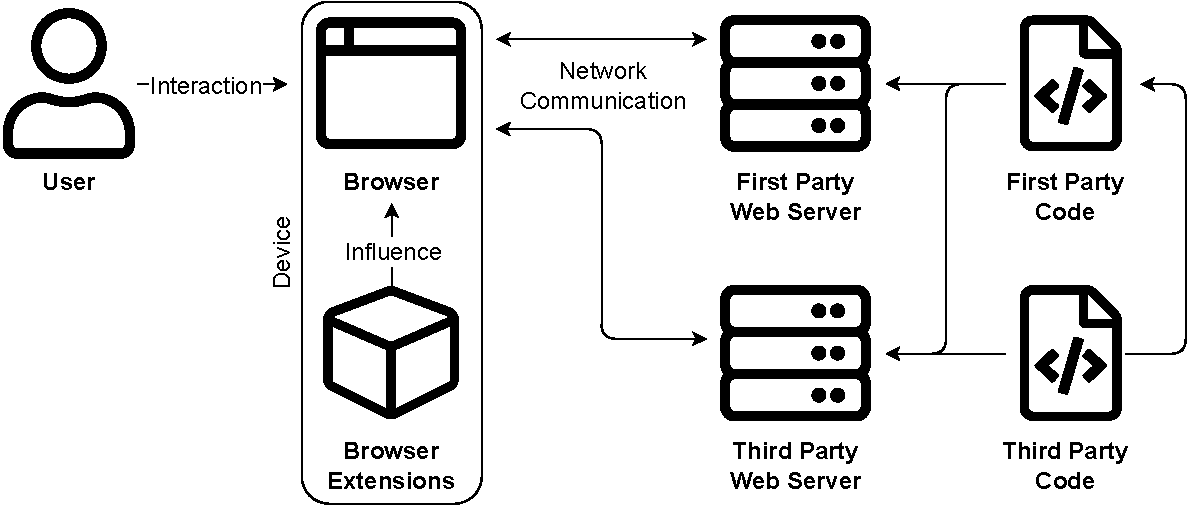
\includegraphics[height=4.5cm]{img/threat-model.pdf}
	\end{center}
	\begin{itemize}
		\item Assume that attacker is able to override APIs
		\item Entry points: XSS, MITM, third-party code/server, extensions
	\end{itemize}
\end{frame}

\begin{frame}
	\frametitle{Threats of API Manipulation}
	\begin{itemize}
		\item Interception and manipulation of requests
		% $\rightarrow$ Application layer DDoS
		\item Access plain-text before encryption
		\item Manipulate PRNG\\
		$\rightarrow$ Compromize generated passwords, tokens, cryptographic keys
		\item Intercept sensitive data and credentials
	\end{itemize}
\end{frame}

\section{Detection and Automated Analysis Tool}

\begin{frame}[fragile]
	\frametitle{Detection of API Manipulation}
	\begin{itemize}
		\item Intercept API Overrides
		\begin{itemize}
			\item Setter function
			\item \texttt{Object.defineProperty(…)}
		\end{itemize}
		\item Verify Integrity
		\begin{itemize}
			\item Store and compare references
			\item Check \texttt{toString()}
		\end{itemize}
\begin{overprint}
\onslide<2>
		\begin{lstlisting}[language=JavaScript,numbers=none,showstringspaces=true]
// Chromium
`function ${name}() { [native code] }`
// Firefox
`function ${name}() {\n    [native code]\n}`
		\end{lstlisting}
\end{overprint}
	\end{itemize}
\end{frame}

\begin{frame}
	\frametitle{Browser Extension} % “WAM Detector”
	\begin{center}
		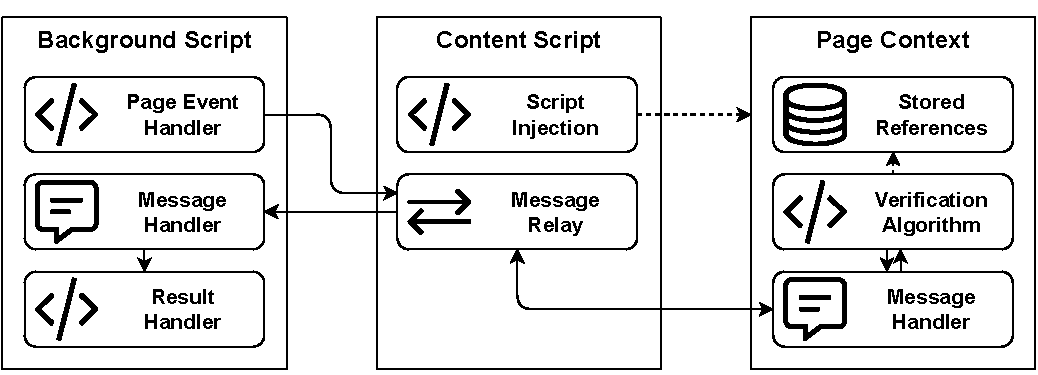
\includegraphics[height=4.5cm]{img/context-diagram.pdf}
	\end{center}
\end{frame}

\begin{frame}
	\frametitle{Automated Analysis}
	\vfill
	\begin{center}
		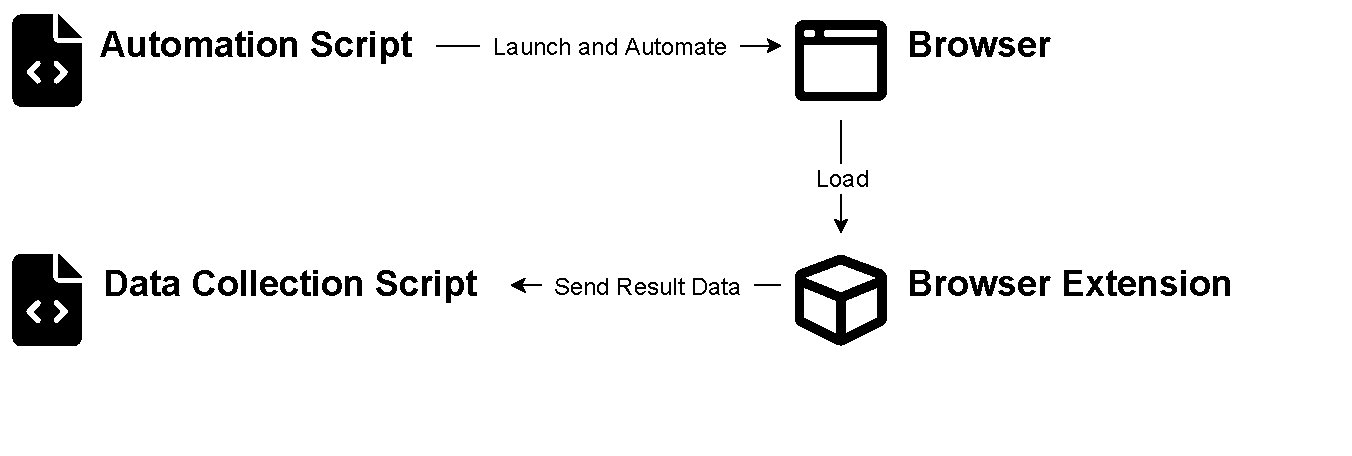
\includegraphics[height=3.6cm]{img/automation-notext.pdf}
	\end{center}
	\vfill
\end{frame}

\begin{frame}[plain]
	%\frametitle{Demonstration}
	\centering
	\vspace*{\fill}
	\usebeamerfont{frametitle}
	\textbf{Demonstration of\\ Browser Extension}
	\vspace*{\fill}
\end{frame}

\section{Evaluation of API Overwriting}

\begin{frame}
	\frametitle{Evaluation of API Overwriting in Popular Websites}
	\begin{itemize}
		\item 16.000 domains from Tranco list
		\item 18 \% failed (CDNs, redirects, …)
		\item APIs commonly overwritten
		\begin{itemize}
			\item 44 \% ~\texttt{history}
			\item 14 \% ~\texttt{fetch}
		\end{itemize}
		\item Tracking, Monitoring
	\end{itemize}
	\raggedleft
	\par\vspace{-3cm}
	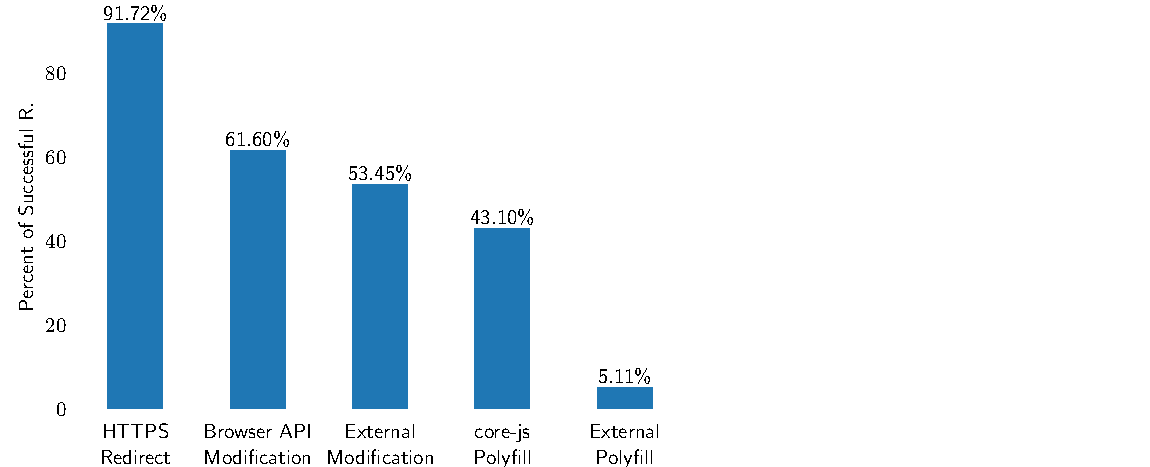
\includegraphics[height=5.5cm]{img/evaluation-overview-bars.pdf}
\end{frame}

\section{Mitigation and Best Practices}

\begin{frame}[fragile]
	\frametitle{Mitigation and Best Practices}
	\begin{itemize}
		\item Reduce the attack surface
		\begin{itemize}
			\item Avoid including external JavaScript + third-party dependencies
			% Some applications might need to use CDNs though => use SRI
			\item Prevent manipulation with Subresource Integrity (SRI)
		\end{itemize}
		\item Content Security Policy (CSP)
		\begin{itemize}
			\item Block resources from untrusted origins
			\item Monitor untrusted inclusions
		\end{itemize}
		\begin{lstlisting}[language=CSP,numbers=none]
default-src 'self'; img-src cdn.example.com; report-uri ...
		\end{lstlisting}
		\item Verify web application behavior
		\begin{itemize}
			\item Use tools such as the browser extension
		\end{itemize}
	\end{itemize}
\end{frame}

\section{Conclusion and Outlook}

\begin{frame}
	\frametitle{Conclusion}
	\begin{itemize}
		\item API overwriting is common
		\item Poses a significant threat
		\item Attacks can be detected and mitigated
	\end{itemize}
\end{frame}

\begin{frame}
	\frametitle{Outlook}
	\begin{itemize}
		\item Reliably classify malicious vs. legitimate
		\item Automate code analysis, scan repositories
		\item Sandboxing built-in to browsers
	\end{itemize}
\end{frame}

\begin{frame}[plain]
	%\frametitle{That's all, folks!}
	\centering
	\vfill
	\usebeamerfont{frametitle}
	Thank you for your attention.
	\par
	Are there any questions?
	\vfill
\end{frame}

\begin{frame}
	\frametitle{Mitigations II}
	\begin{itemize}
		\item Only overwrite browser APIs when necessary
		\item Configure HTTPS with secure settings
		\item Honor \texttt{Upgrade-Insecure-Requests} header
		\item Automated scanning of web applications
	\end{itemize}
\end{frame}

\begin{frame}
	\frametitle{Mitigations III - Advice for Users}
	\begin{itemize}
		\item Detect manipulation with browser extension
		\item Block malicious resources, eg. with uBlock Origin, uMatrix
		\begin{itemize}
			\item ADs increase the attack surface % (when not properly sandboxed)
			\item Trackers commonly overwrite browser APIs
		\end{itemize}
	\end{itemize}
\end{frame}

\end{document}